\documentclass{beamer}
\usepackage[utf8]{inputenc}
\usepackage{graphicx}

% themes found here: https://latex-beamer.com/tutorials/beamer-themes/
% \usetheme{PaloAlto}
\usetheme{CambridgeUS}
\setbeamertemplate{footline}[frame number]

% name t.b.d.
\title{Resilient Weather Kriging}

\author{
    Baxter, Hunter %\\
    \and
    Callandriello, Meghan
    \and
    Hicks, Jaden
    \and
    Pena, Alex
}

\begin{document}
\maketitle


\begin{frame}{Main Idea}
\begin{itemize}
    \item The goal of our project is not as much about the specific weather data
    but rather to work on solving a problem focused on principled software engineering practices. 
    % mention why real time weather data matters (ex. road conditions, agriculture) 
    \item In particular, the type of data we will be working with is spatio-temporal data.
    \item Our objective is to fill sparsity of data over a geographic area, as one can imagine being in a scenario where one does not have access to an infinite supply of sensors. 
    % acknowledge that this is just a demonstration of spatio-temporal data, not that weather is a cutting edge problem
    \item Due to the ease of access of current weather data, we are using weatherbit as a data vendor
    % spatio-temporal data has sweet visualizations so it offers something to everyone
\end{itemize}
\end{frame}

\begin{frame}{Architecture}
% update with latest architecture
\begin{center}
    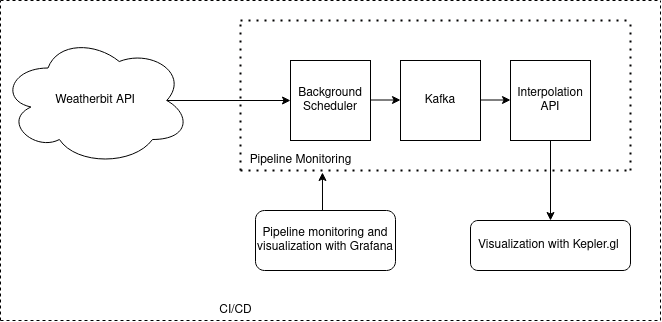
\includegraphics[width=.6\linewidth]{figures/architecture.png}
\end{center}
\end{frame}

\begin{frame}{Resilient?}
\begin{itemize}
    \item A system is resilient if it continues to carry out its mission in the face of adversity
    \item Although we can not achieve perfect resiliency, we can employ strategies to allow it. 
\end{itemize}    
\end{frame}

\begin{frame}{CI/CD}
\begin{itemize}
    \begin{columns}
    \begin{column}{0.4\textwidth}
    \item Current version one uses \textbf{Github Actions} for Continuous Integration
    \vspace{1cm}
    \item Version two will use \textbf{Jenkins} for continuous integration and deployment
    \end{column}
    \begin{column}{0.4\textwidth}
    \begin{center}
    
\includegraphics[width=0.5\linewidth]{figures/github_actions.png} \\
    
\includegraphics[width=0.5\linewidth]{figures/jenkins_icon.png} \\
    \end{center}
    \end{column}
    \end{columns}
    % pls give me feedback if y'all want to have this slide in presentation or we can get to 5 min easily
    % TODO: describe why it is industry grade
    % explain goal is to use a shrunken scope to get familiar with tool similarly to our PA
\end{itemize}
\end{frame}

\begin{frame}{Backend}
% note: need to describe why it is resilient with these
% docker swarm (we might just want to use k8 since it has more source code) 
% kafka
% scheduler
\begin{itemize}
    \item In order to create a resilient system, we have containerized all of our services using Docker. 
    \item In the event that any service goes offline or fails, the container will be restarted via Docker Swarm. 
    \item We have implemented a background scheduler which will request current information from the Weatherbit API every 30 minutes. This data will be published to Kafka brokers where each topic is defined by the weather station which provided the data. 
\end{itemize}
\end{frame}

\begin{frame}{Frontend}
\begin{itemize}
    \item Even though the weatherbit data we are using will be streamed in real time, the  visualization of the weather will going to be on demand. 
    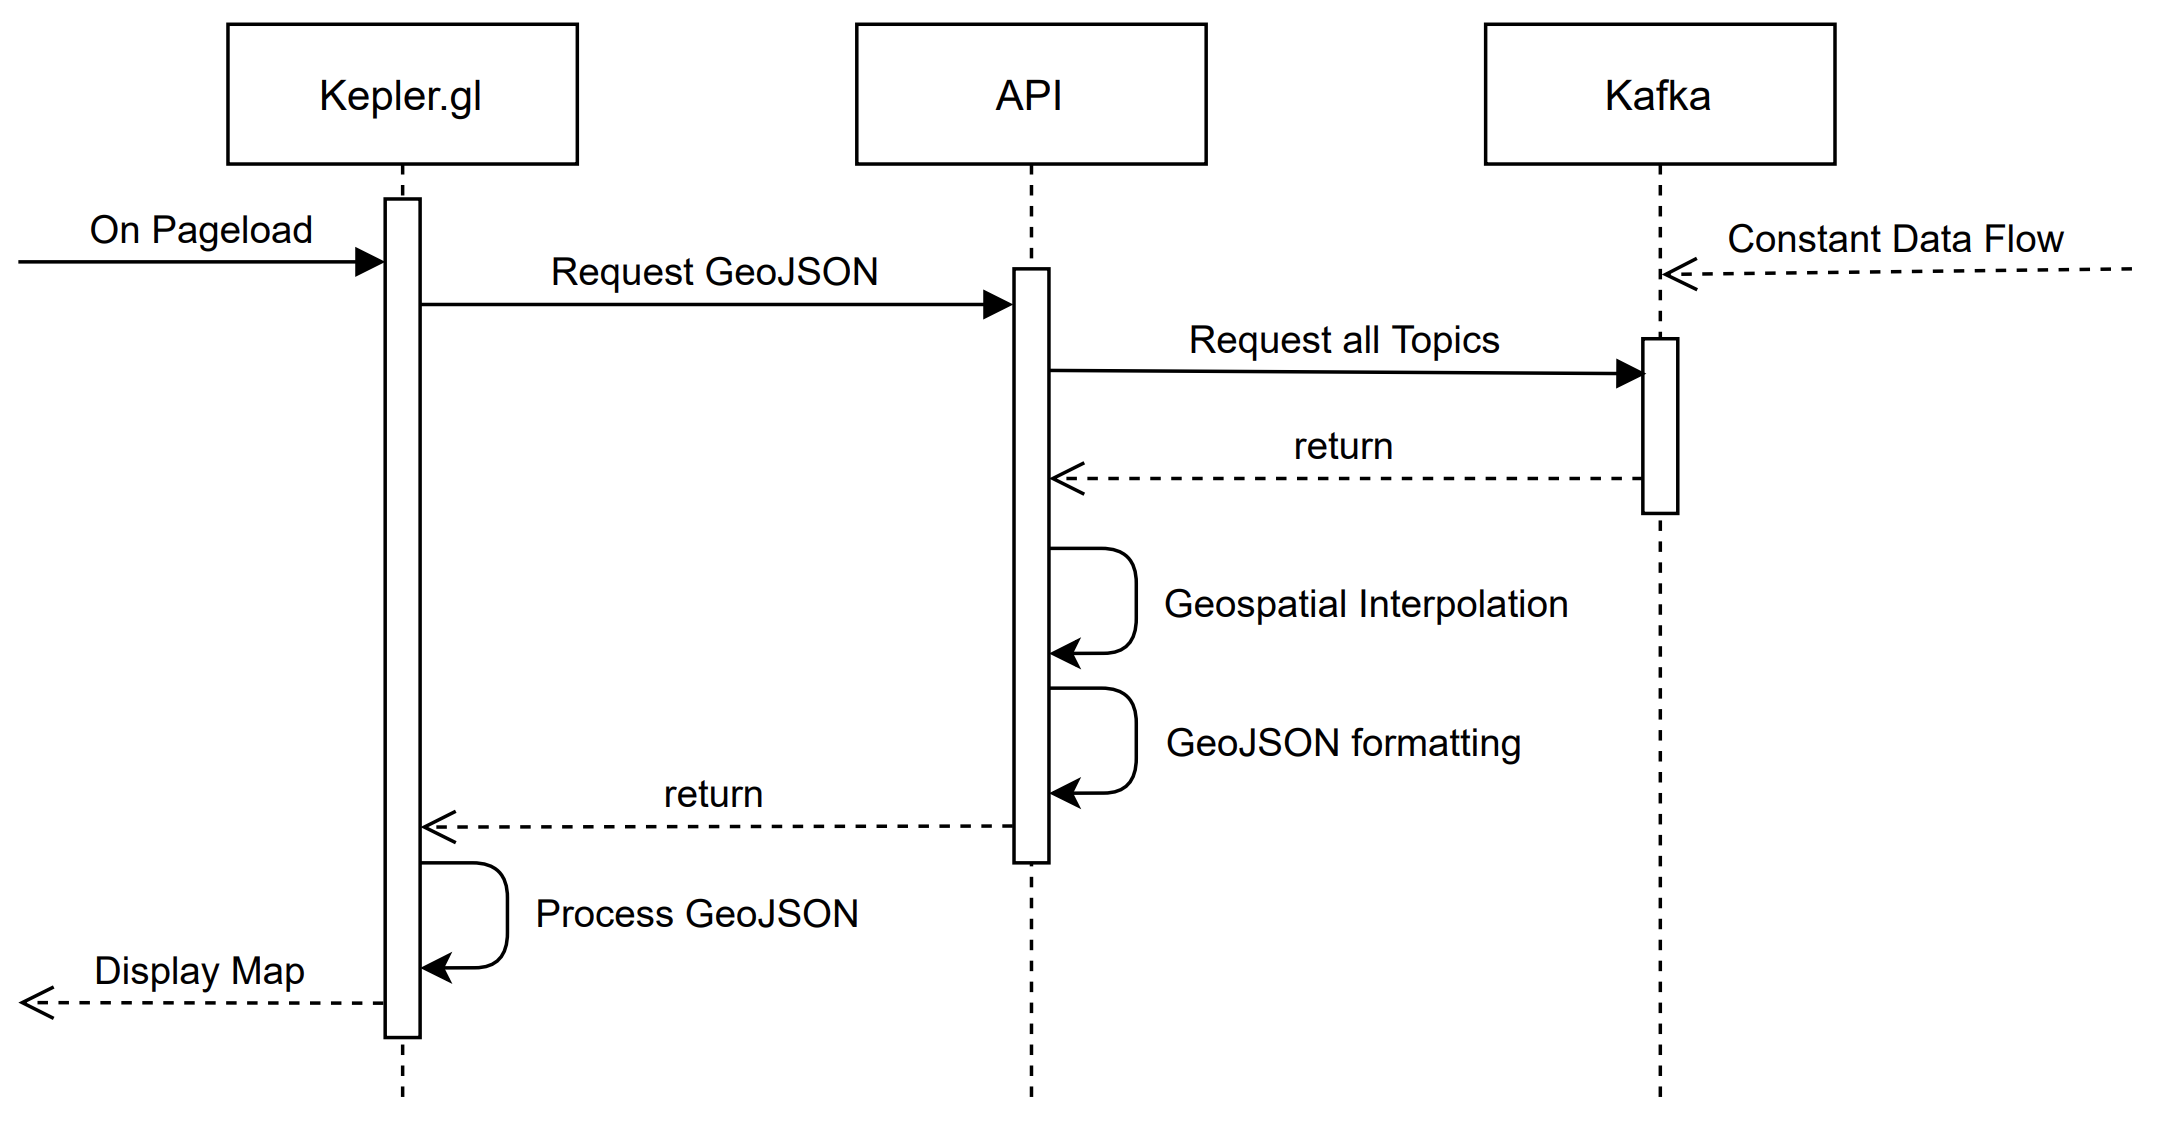
\includegraphics[width=.9\linewidth]{figures/Frontend_Flow.png}
\end{itemize}
\end{frame}

% hunter needs to work on wording in morning since he is tired
\begin{frame}{Geospatial Interpolation}
Due to the aforementioned sparsity over a geographical region,
we will be using a statistical technique due to the hypothetical problem that there are a limited amount of data sources available over a geographical region
% this is where we can acknowledge that weather does not necessarily have this problem anymore, but being clever with interpolation strategies can reduce costs
\begin{center}
    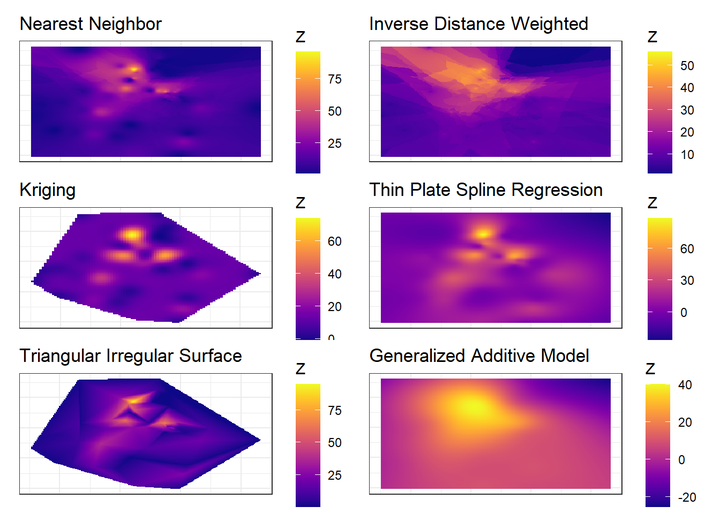
\includegraphics[width=0.65\linewidth]{figures/geostats.png} \\
\end{center}
\end{frame}

\begin{frame}{Dummy Frame}
\begin{itemize}
    \item bullet points are easy
    why is this sentence on same line? 
    \item \textbf{I am bold} \\
    why is this one not on same line? because I used "\textbackslash \textbackslash"
    \item \textit{I am italicized}
    \item \underline{I am underlined}
\end{itemize}
\end{frame}

\begin{frame}{kepler.gl}
% insert kepler.gl front-end application information
\begin{itemize}
    \item To visualize the results of interpolation, we are using kepler.gl, an open-source visualization tool developed specifically for geospatial data sets. 
    \item React has libraries that support kepler.gl, making it possible to embed live visualizations in a react web-application.
\end{itemize}
\begin{center}
    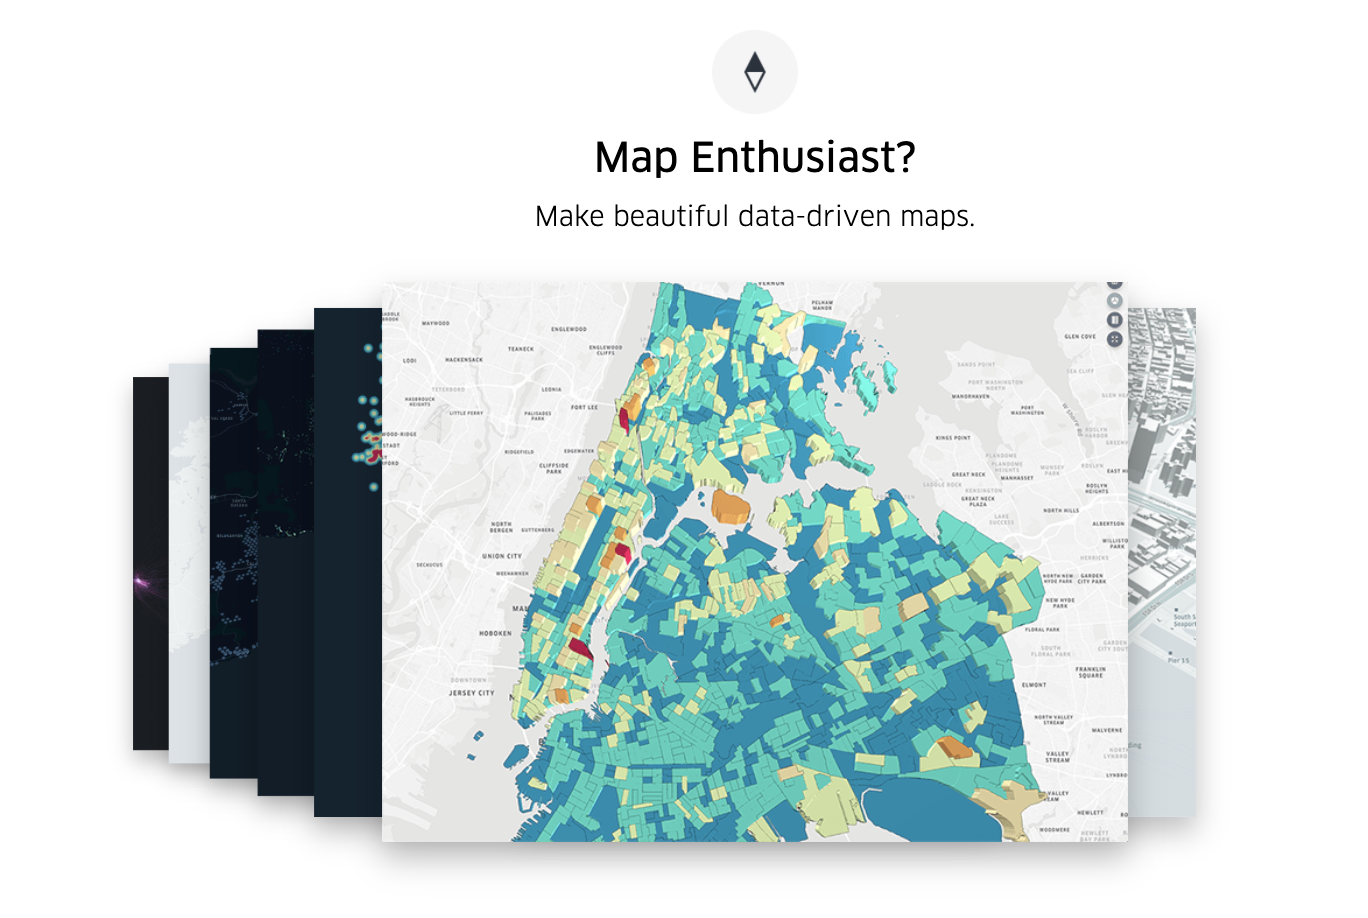
\includegraphics[width=0.60\linewidth]{documentation/project_presentation/figures/Kepler.png} \\
\end{center}
\end{frame}

\end{document}